\documentclass[12pt]{article}
\renewcommand{\baselinestretch}{1.2}
\usepackage[utf8]{vietnam}
\usepackage[a4paper, total={6in, 8in}]{geometry}
\usepackage[english]{babel}
\usepackage{hyperref}
\usepackage{mathtools}
\usepackage{amssymb}
\usepackage{indentfirst}
\usepackage{graphicx}
\usepackage{minted}
\usepackage{ragged2e}
\usepackage{multirow}
\usepackage{subcaption}
\usepackage{xurl}
\usepackage{amsmath}
\usepackage{makecell}
\usepackage{algorithm}
\usepackage{algpseudocode}
\renewcommand\theadalign{bc}
\renewcommand\theadfont{\bfseries}
\renewcommand\theadgape{\Gape[4pt]}
\renewcommand\cellgape{\Gape[4pt]}
\usepackage{pbox}
\usepackage{graphicx}
\usepackage{diagbox}
\usepackage{listings}
\usepackage{xcolor}

\hypersetup{
    colorlinks=true,
    linkcolor=blue,
    citecolor=blue,
    urlcolor=blue,
}
\lstset{
    backgroundcolor=\color{white},   
    basicstyle=\footnotesize,       
    breakatwhitespace=false,         
    breaklines=true,                 
    captionpos=b,                    
    commentstyle=\color{red},    
    escapeinside={\%*}{*)},          
    extendedchars=true,              
    keepspaces=true,                 
    keywordstyle=\color{blue},       
    language=Python,                
    numbers=left,                    
    numbersep=5pt,                  
    showspaces=false,                
    showstringspaces=false,
    showtabs=false,                  
    tabsize=2
}
\begin{document}
\begin{center}
    \vspace*{1.8cm}
    \Large
    Project\\
    Advanced Programming for HPC\\
    Nguyen Thi Ly Linh (M22.ICT.003)\\
    November 5th 2023\\
\end{center}

\section{Input}
I have used an original image with width=1280 and height=960
\begin{figure}[H]
\centering
    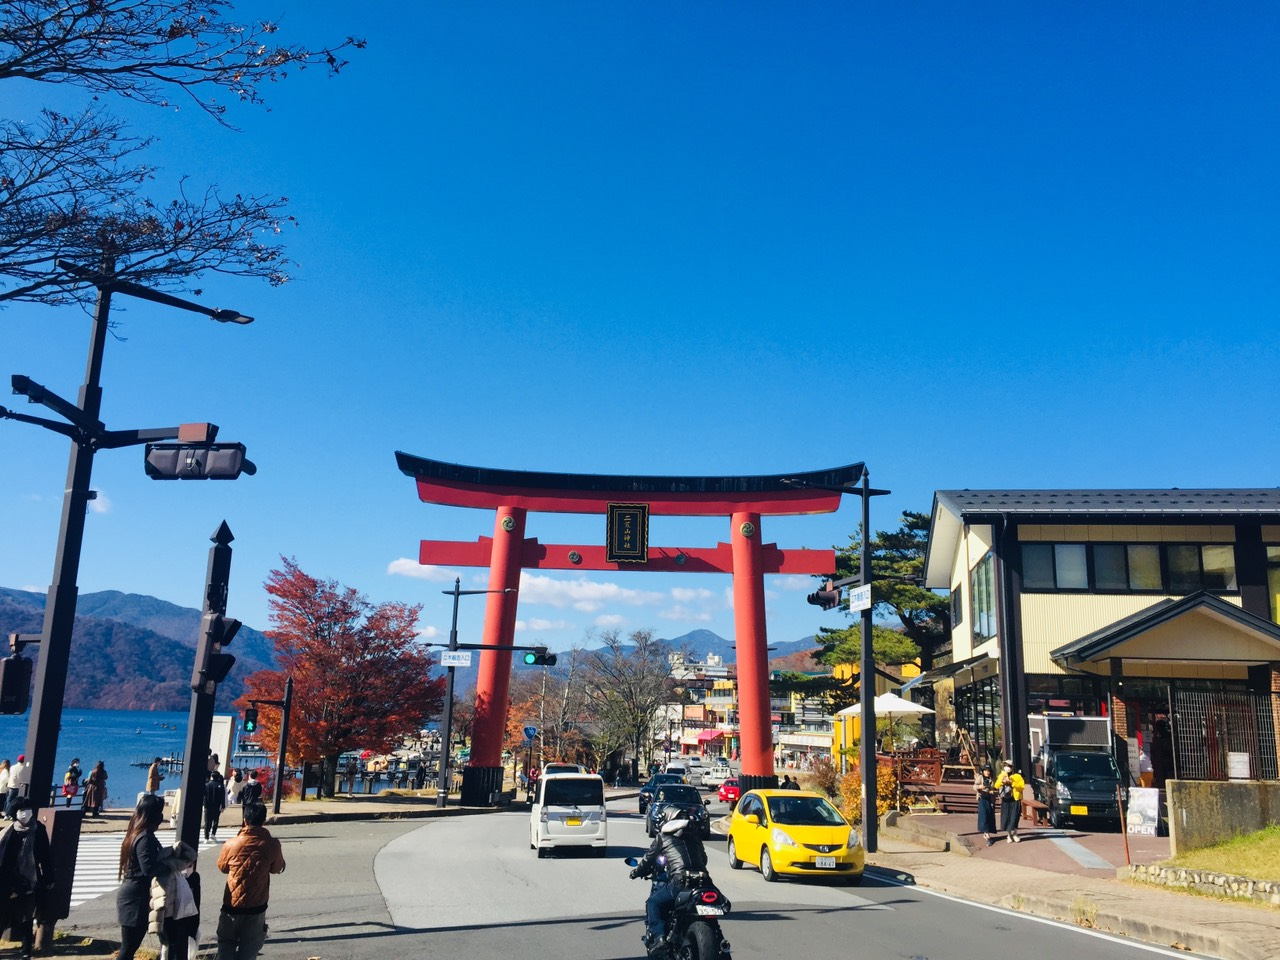
\includegraphics[height = 0.5\textheight, keepaspectratio]{images/kuwahara.jpg}
    \caption{The original image}
\end{figure}
\section{Implementation}
To implement the Kuwahara filter, I have executed the main following four steps.
\begin{itemize}
    \item Step 1: Convert RGB to HSV.
    \item Step 2: Calculate the mean and variance for each channel of four corners.
    \item Step 3: Determine the quadrant with the minimum variance.
    \item Step 4: Set the pixel value to the mean of the channel in the minimum variance quadrant.
\end{itemize}
\subsection{Program}
\begin{enumerate}
    \item Step 1: Convert RGB to HSV.
    \begin{lstlisting}[language=Python]
@cuda.jit
def rgb_to_hsv(src, dst):
    x, y = cuda.grid(2)
    if y < dst.shape[0] and x < dst.shape[1]:
        max_value = max(src[y, x, 0], src[y, x, 1], src[y, x, 2])
        min_value = min(src[y, x, 0], src[y, x, 1], src[y, x, 2])
        delta = max_value - min_value
        if delta == 0:
            h_value = 0
        elif max_value == src[y, x, 0]:
            h_value = 60 * (((src[y, x, 1] - src[y, x, 2]) / delta) % 6)
        elif max_value == src[y, x, 1]:
            h_value = 60 * (((src[y, x, 2] - src[y, x, 0]) / delta) + 2)
        elif max_value == src[y, x, 2]:
            h_value = 60 * (((src[y, x, 0] - src[y, x, 1]) / delta) + 4)

        if max_value == 0:
            s_value = 0
        else:
            s_value = delta / max_value
        v_value = max_value
        dst[y, x, 0] = h_value
        dst[y, x, 1] = s_value
        dst[y, x, 2] = v_value  
    \end{lstlisting}
    \item Step 2: Calculate the mean and variance for each channel of four corners.
    \begin{lstlisting}[language=Python]
 for c in range(0,3):
    channel_values = neighborhood[:, :, c]
    channel_values_rgb = neighborhood_rgb[:, :, c]
    mean = 0.0
    mean_rgb = 0.0
    variance = 0.0
    size = neighborhood.shape[0]*neighborhood.shape[1]
    # Calculate the mean
    for i in range(neighborhood.shape[0]):
        for j in range(neighborhood.shape[1]):
            mean += channel_values[i, j]
    mean //= size

    for i in range(neighborhood_rgb.shape[0]):
        for j in range(neighborhood_rgb.shape[1]):
            mean_rgb += channel_values_rgb[i, j]
    mean_rgb //= size

    # Calculate the variance
        for i in range(neighborhood.shape[0]):
            for j in range(neighborhood.shape[1]):
                variance += (channel_values[i, j] - mean) ** 2

    variance /= size
    mean_variances[q, c] = variance
    mean_variances[q, c +3] = mean
    mean_variances[q, c +6] = mean_rgb
    \end{lstlisting}
    \item Step 3: Determine the quadrant with the minimum variance.
    \begin{lstlisting}[language=Python]
min_variance_quadrant = 0
min_variance =math.sqrt( mean_variances[0, 0] + mean_variances[0, 1] + mean_variances[0, 2])

for q in range(1, 4):
    nn =math.sqrt( mean_variances[q, 0] + mean_variances[q, 1] + mean_variances[q, 2])
    if nn < min_variance:
        min_variance_quadrant = q
        min_variance = nn
    \end{lstlisting}
    \item Step 4: Set the pixel value to the mean of the channel in the minimum variance quadrant.
    \begin{lstlisting}[language=Python]
output_image[x, y, 0] = mean_variances[min_variance_quadrant, 6]
output_image[x, y, 1] = mean_variances[min_variance_quadrant, 7]
output_image[x, y, 2] = mean_variances[min_variance_quadrant, 8]
    \end{lstlisting}
\end{enumerate}
\subsection{Result}
The output images on CPU and GPU with shared memory and without shared memory are as below.
\begin{figure}[H]
\centering
    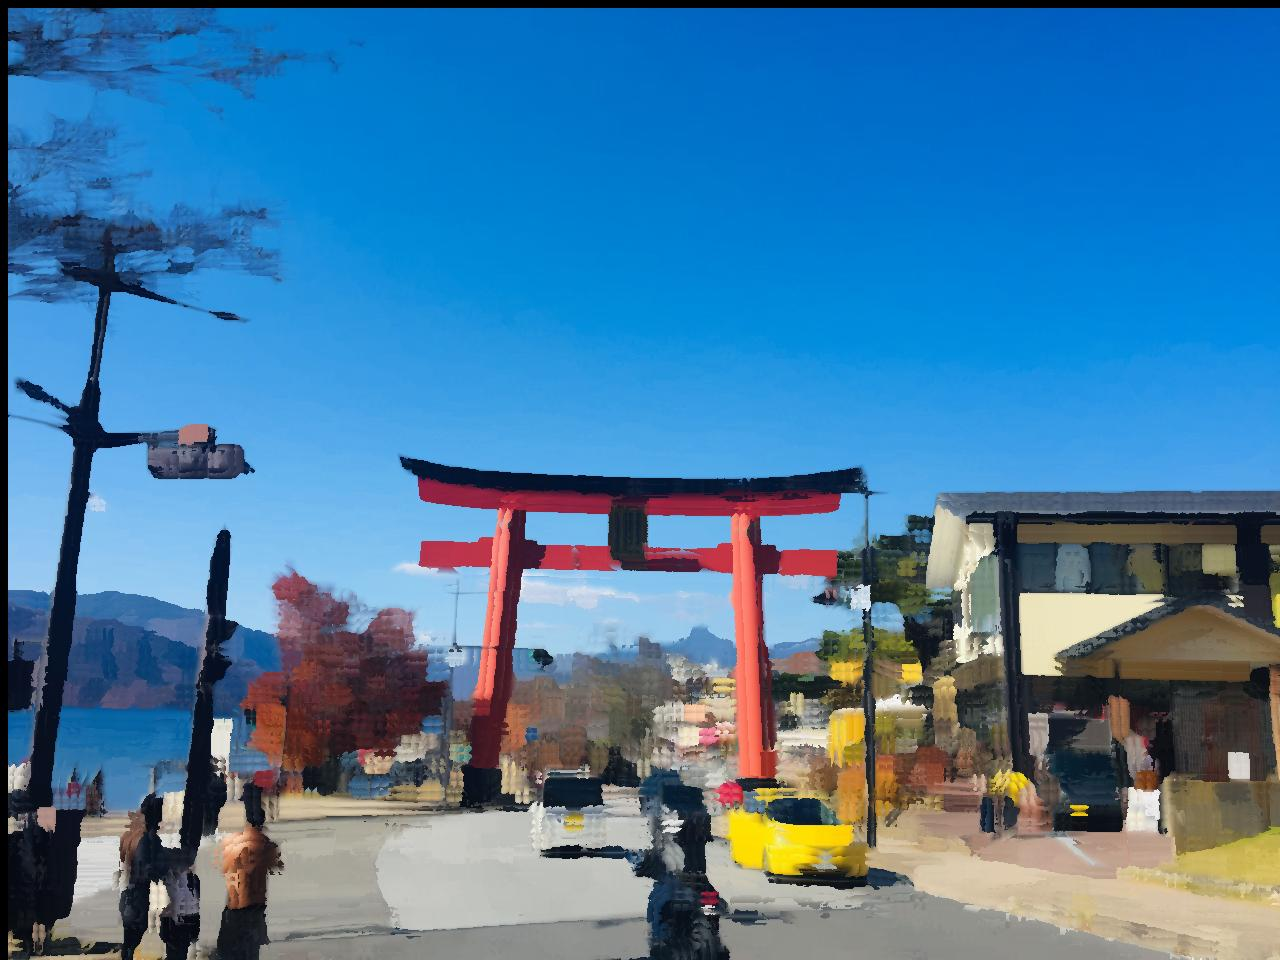
\includegraphics[height = 0.5\textheight, keepaspectratio]{images/kuwahara_windowsize_8__without_sm.jpg}
    \caption{The output image \textbf{in CPU} - window size 8}
\end{figure}
\begin{figure}[H]
\centering
    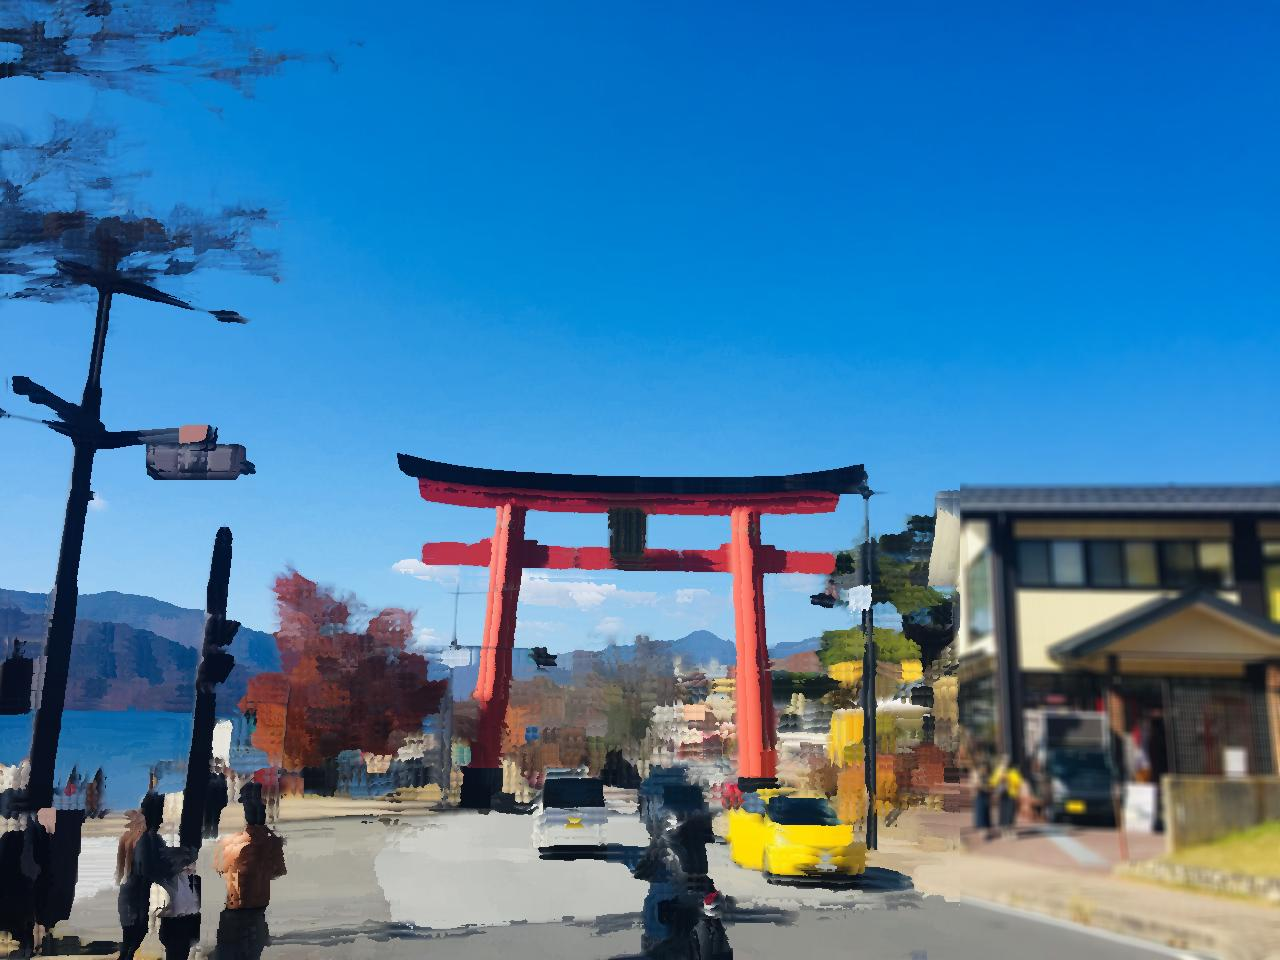
\includegraphics[height = 0.5\textheight, keepaspectratio]{images/kuwahara_windowsize_8_blocksize_(8,8)_with_sm.jpg}
    \caption{The output image \textbf{in GPU} - window size 8 with shared memory}
\end{figure}
\begin{figure}[H]
\centering
    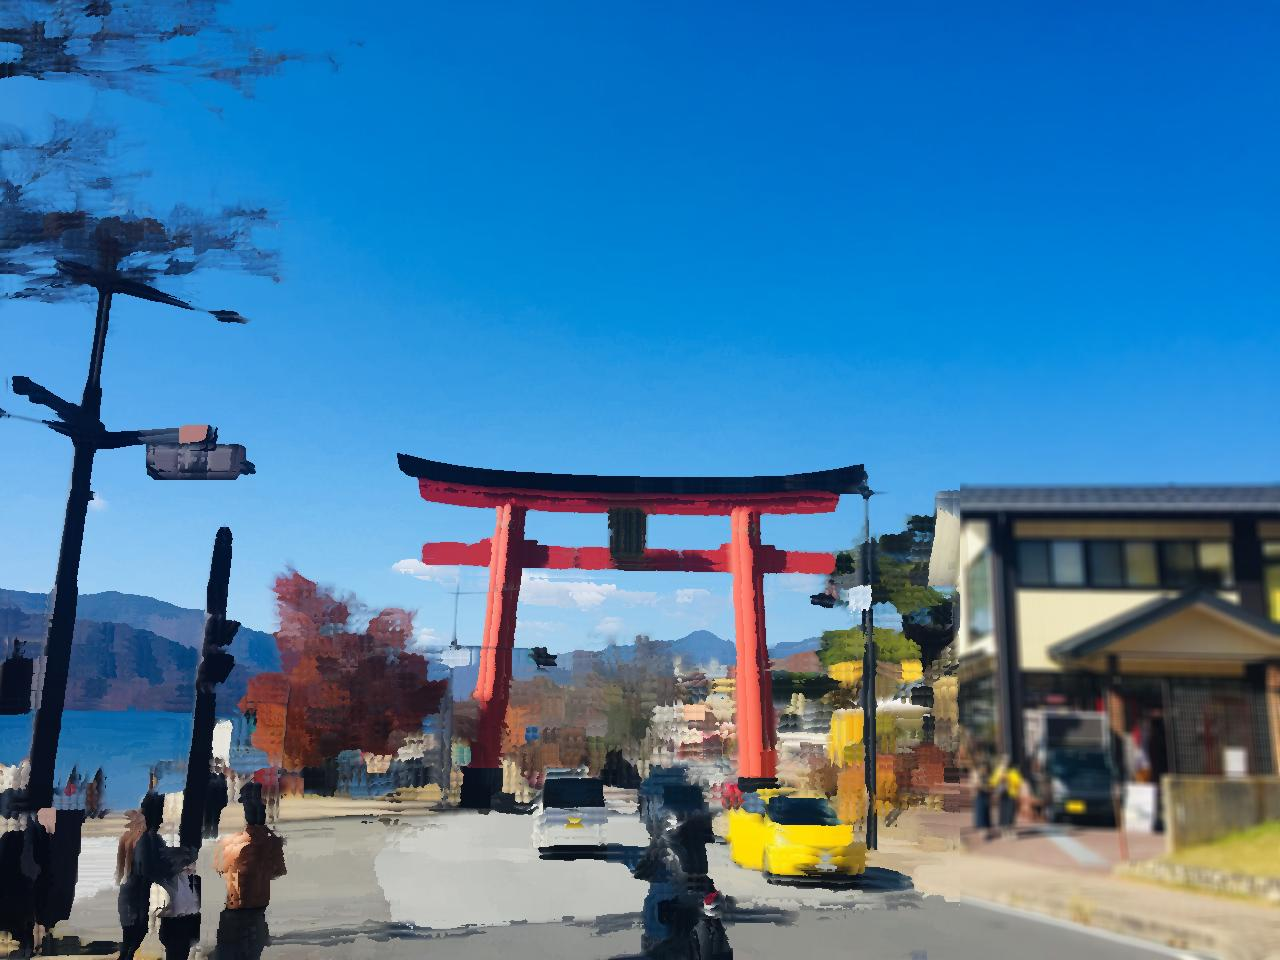
\includegraphics[height = 0.5\textheight, keepaspectratio]{images/kuwahara_windowsize_8_blocksize_(8,8)__without_sm.jpg}
    \caption{The output image \textbf{in GPU} - window size 8 without shared memory}
\end{figure}
\subsection{Execution time}
\begin{table}[H]
    \centering
    \begin{tabular}{|c|c|c|c|c|c|}
        \hline
         & Window size 5 & Window size 6 & Window size 7 & Window size 8 \\ 
        \hline
        CPU  & 433.6351 & 571.8690 & 735.6915 & 918.3598\\ 
        \hline
    \end{tabular}
    \caption{Execution time in \textbf{CPU } on different window sizes}
    \label{tab:mytable}
\end{table}

\begin{table}[H]
    \centering
    \begin{tabular}{|c|c|c|c|c|c|}
        \hline
         & Window size 5 & Window size 6 & Window size 7 & Window size 8 \\ 
        \hline
        GPU Block size (2,2) & 1.2011 & 0.0012 & 0.0006 & 0.0011\\ 
        \hline
        GPU Block size (4,4) & 0.0011 & 0.0011 & 0.0011 & 0.0010\\ 
        \hline
        GPU Block size (8,8) & 0.0010 & 0.0012 & 0.0049 & 0.0010\\ 
        \hline
    \end{tabular}
    \caption{Execution time in \textbf{GPU without shared memory} on different window sizes and block sizes}
    \label{tab:mytable}
\end{table}

\begin{table}[H]
    \centering
    \begin{tabular}{|c|c|c|c|c|c|}
        \hline
         & Window size 5 & Window size 6 & Window size 7 & Window size 8 \\ 
        \hline
        GPU Block size (2,2) & 0.8776 & 0.0011 & 0.0045 & 0.0012\\ 
        \hline
        GPU Block size (4,4) & 0.0013 & 0.0004 & 0.0011 & 0.0009\\ 
        \hline
        GPU Block size (8,8) & 0.0022 & 0.0004 & 0.0010 & 0.0011\\ 
        \hline
    \end{tabular}
    \caption{Execution time in \textbf{GPU with shared memory} on different window sizes and block sizes}
    \label{tab:mytable}
\end{table}

\section{Discussion}
I have tried to implement in CPU and GPU with different block sizes and different window sizes in several time and have the following summarise.
\begin{itemize}
    \item In CPU, it takes a lot of time to process large size images. Especially, when we increase the window sizes, the execution time also increases. Therefore, we should think about the solution in GPU. It can improve the speed a lot.
    \item In GPU, the first time is always slower than the next times because it takes a lot of time for initiation.
    \item In GPU, the speed increases if we increase the block sizes.
    \item In GPU with this filter, the speed with shared memory and without shared memory are almost the same.
    \item In GPU, when we increase the window size, the speed does not change a lot. However, the output images have more efficiency on Kuwahara filter.
\end{itemize}
\section{Future work}
There are two things that have been left for the future due to lack of time.
\begin{itemize}
    \item In CPU, explanation why the output images have black border on two edges (above and left sight).
    \item In GPU, optimization.
\end{itemize}
\end{document}